\begin{frame} \frametitle{\vspace*{0.5cm}DUS-induced lung hemorrhage is not a new problem}
  {\small%
    \begin{itemize}%
    \item Lung Hemorrhage (LH) is the only known bioeffect of non-contrast DUS%
    \item Has been shown to occur in mice, rats, pigs, rabbits, monkeys \citep{Child1990,OBrien1997a,Tarantal1994a}.%
    \item DUS-induced LH does not appear to be a result of cavitation or heating.%
    \item The underlying physical damage mechanism is not understood.%
    \end{itemize}%
    % 
    \begin{figure}%
      \centering%
      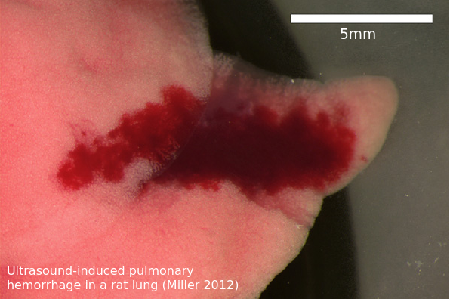
\includegraphics[width=0.5\textwidth]{LungBleed2} \nocite{Miller2012}%
    \end{figure}%
    %
    The basic physical problem we have in the lungs is a mechanical wave interacting with an air-tissue interface.
    %\visible<2>{We aim to use computational modeling and simulations to investigate the underlying physics of DUS-induced LH.}%
    % 
  }
  \note{
    \begin{enumerate}
    \item DUS-induced LH isn't new.
    \item Has been shown to occur under clinically safe conditions in a variety of mammals
    \item Isn't a result of typical US bioeffect mechanisms
    \item Physical damage mechanism isn't understood.
    \end{enumerate}
  }
\end{frame}

%%% Local Variables:
%%% mode: latex
%%% TeX-master: "../main"
%%% End:
